%% tez.tex
%% Copyright 2015 Gökçe Mehmet AY
%
% This work may be distributed and/or modified under the
% conditions of the LaTeX Project Public License, either version 1.3
% of this license or (at your option) any later version.
% The latest version of this license is in
%   http://www.latex-project.org/lppl.txt
% and version 1.3 or later is part of all distributions of LaTeX
% version 2005/12/01 or later.
%
% This work has the LPPL maintenance status `maintained'.
% 
% The Current Maintainer of this work is Gökçe Mehmet AY.
%
% This work consists of the files esogu.cls and tez.tex




% Şablon otomatik olarak kapak ve onay sayfalarını sizin esogu.cls dosyasında girdiğiniz bilgilere göre oluşturmaktadır. Lütfen o dosyadaki "TEZLE İLGİLİ Bilgileri burada giriniz." bölümünü doldurunuz. 

% Eğer Tezinizi bu dosyada yazacaksanız "TEZİNİZİ BURADAN SONRA EKLEYİNİZ" bölümünden sonra ekeleyebilirsiniz. Özet ve Summary bölümleri /bolum klasörünün içindedir. 





\documentclass[]{esogu}			% Optionlar boş olacak, şablonu kullanmak için
\usepackage{lipsum}				% Örnek tezde anlamsız metin yazmak için bu paket gerekli. Tezinizde bu bölümü silebilirsiniz. 

\bibliography{kaynakca.bib}		% Kaynakça dosyası için Bunu Zotero, Mendeley, Endnote ya da CiteU gibi bir programla oluşturmanızı tavsiye ederim. Zotero hakkında bilgi http://makina.gmay.me/Bulutta/ adresindeki ekitapta mevcut.

%----------------------------------------------------------------------------------------
\begin{document}

\frontmatter %roma rakamları ile yazdırmak için
\title{OGU deneme}
%-----Dış kapak Türkçe---------- Burayı değiştirmeyin
\begin{titlingpage*}
\begin{center}
\footnotesize


	\begin{vplace}							% Metni ortalamak için
	\large									%tezbaşlığını büyük yazmak için
	\tbaslik\\								% Tez başlığı
	\footnotesize							% 10 puntoya düş

	\vspace{1pc}
	\yazar	\\								% yazar ismi
	\vspace{1pc}
	\textbf{\unvan\space TEZİ}\\
  	\vspace{1pc}
	\bolum \space Anabilim Dalı\\
	\vspace{1pc}
	\teslim\\
	\end{vplace}
\end{center}

\end{titlingpage*}
%----------------------------------------------------------------------
%-----Dış kapak İngilizce-----Burayı değiştirmeyin-----
\begin{titlingpage*}
\begin{center}
\footnotesize


	\begin{vplace}							% Metni ortalamak için
	\large									%tezbaşlığını büyük yazmak için
	\tbasliken\\								% Tez başlığı
	\footnotesize							% 10 puntoya düş

	\vspace{1pc}
	\yazar	\\								% yazar ismi
	\vspace{1pc}
	\textbf{\unvanen\space THESIS}\\
  	\vspace{1pc}
	\bolumen \space Department\\
	\vspace{1pc}
	\teslimen\\
	\end{vplace}
\end{center}

\end{titlingpage*}
%----------------------------------------------------------------------
%	iç Kapak Burayı değiştirmeyin
%----------------------------------------------------------------------------------------

\begin{titlingpage*}
\begin{center}
\footnotesize
\begin{vplace}							% Metni ortalamak için
\tbaslik\\								% Tez başlığı
\vspace{7pc}							% 12 punto 7 boşluk için
\yazar	\\								% yazar ismi
\vspace{7pc}							% 12 punto 7 boşluk için
Eskişehir Osmangazi Üniversitesi\\		
Fen Bilimleri Enstitüsü\\
Lisansüstü Yönetmeliği Uyarınca\\
\bolum \space Anabilim Dalı\\
\bilim \space Bilim Dalı\\
\unvan \space TEZİ\\
Olarak Hazırlanmıştır\\
\vspace{7pc}
Danışman:\space \danisman\\			
\vspace{2pc}
\proje\\ 								%Varsa proje kapsamında desteklenip desteklenmediği buraya yazılacak
\end{vplace}

\vfill
\teslim\\
\vspace{2cm}
\end{center}

\end{titlingpage*}
\normalsize

%----------Onay--------------
\thispagestyle{empty}
\begin{center}
\large
\textbf{ONAY} 
\normalsize
\end{center}
\bolum \space Anabilim Dalı \unvan \space öğrencisi \yazar \space tezi olarak hazırladığı "\textbf{\tbaslik}" başlıklı bu çalışma, jürimizce lisansüstü yönetmeliğin ilgili maddeleri uyarınca değerlendirilerek kabul edilmiştir.

\noindent \textbf{Danışman}\space\space\space\space\space\space\space\space:\space \danisman 

\noindent \textbf{İkinci Danışman}\space:\space \ikidanisman
\newline

\noindent \textbf{Doktora Tez Savunma Jürisi:}

\noindent \textbf{Üye :\space}\jbir

\noindent \textbf{Üye :\space}\jiki

\noindent \textbf{Üye :\space}\juc

\noindent \textbf{Üye :\space}\jdort

\noindent \textbf{Üye :\space}\jbes


\begin{framed}
Fen Bilimleri Enstitüsü Yönetim Kurulu'nun ........................ tarih ve  \space \space \space \space \space\\................... sayılı kararıyla onaylanmıştır. 
\newline
\newline
\begin{flushright}
\mudur \hspace{1cm}

Enstitü Müdürü\space \space \space \space \space \space \space \space \space \space \space \space \space  %Düzeltilecek ***Biliyorum çok kötü ama hspace çalışmadı
\end{flushright}

\end{framed}


%-------------------Şekiller ve Çizelgeler Dizini----------------
\renewcommand{\listfigurename}{Şekiller Dizini}
\renewcommand{\listtablename}{Çizelgeler Dizini}


\chapter{Etik Beyan}
\begin{center}
\Large\textbf{ETİK BEYAN}
\end{center}
\normalsize
\vspace{3cm}

Eskişehir Osmangazi Üniversitesi Fen Bilimleri Enstitüsü tez yazım kılavuzuna göre, \danisman\space danışmanlığında hazırlamış olduğum “\textbf{\tbaslik}” başlıklı tezimin özgün bir çalışma olduğunu; tez çalışmamın tüm aşamalarında bilimsel etik ilke ve kurallara uygun davrandığımı; tezimde verdiğim bilgileri, verileri akademik ve bilimsel etik ilke ve kurallara uygun olarak elde ettiğimi; tez çalışmamda yararlandığım eserlerin tümüne atıf yaptığımı ve kaynak gösterdiğimi ve bilgi, belge ve sonuçları bilimsel etik ilke ve kurallara göre sunduğumu beyan ederim.   …/…/20…
\vspace{3cm}

\begin{flushright}
\yazar
\end{flushright}
\clearpage

%Özette tez çalışmasının amacı, kapsamı, kullanılan yöntemler ve varılan sonuçlar açık ve öz olarak belirtilmeli, bunlar alt başlıklar altında sunulmamalıdır.  Özetin uzunluğu 250 kelimeyi geçmemelidir. 

%Summary sayfasının içeriği ve düzeni tümüyle Özet sayfasının aynı olmalı ve (vii) ile numaralanmalıdır.

%Özet ve Summary’nin altına anahtar kelimeler/keywords yazılmalıdır.  Konu literatürde hangi kelimelerle geçiyorsa anahtar kelime olarak bu kelimeler kullanılmalıdır.

\chapter{Özet}


fdasgraeg
\chapter{Summary}
\chapter{Teşekkür}



\tableofcontents
\newpage
\listoffigures
\newpage
\listoftables

\clearpage


\mainmatter %arap harfleri ile yazdırmak için
% AltBölüm numaralaması
\setcounter{secnumdepth}{5} % 5 derine kadar numara ver.
%\setsecnumdepth{subsubsection}
%---------TEZİNİZİ BURADAN SONRA EKLEYİNİZ-----------------



\chapter{Giriş}
\lipsum
\section{Giriş 2}
\lipsum 
\subsection{Giriş 3}
				% Metni dosyadan çağırmak için örnek
\chapter{Literatür Araştırması}					% Metni main.tex dosyasında yazmak için örnek
\lipsum 
\chapter{Bulgular ve Tartışma}		% Konu başlığını ve bir kaç satırı main.tex dosyasında yazıp kalanları dış dosyadan almak için örnek. 
Ğ Ş İ gna-gtjsnthjnjfg frakıgnre. gırengğoehnttodgn. gnteıhnrewğhton. nnıdgeantğ. kkkkkk kkkkkk kkkk   kkkkkk kkkkkk kkkkk kkkk kkk kkkkk kkkkkk kkkkkkkk kkkkkk  kkkkkk kkkkkk kkk kkk kkkk kkk kkkk.jkjjj jjjjjj jjjjjjjjjjL 
\chapter{BULGULAR VE TARTIŞMA}

Basit iki terimle \acrfull{OBEB} ve \acrfull{OKEK} kısaltmaları anlatabiliriz. İster kısaltmasını \acrshort{OBEB}, isterseniz de uzun açılımını \acrlong{OKEK} yazdırabilirsiniz. Bunu yapabilmek için dosyanın başında terimleri tanımlamanız gereklidir. İsterseniz matematik terimlerini de, örneğin \acrshort{pi} böyle tanımlayabilirsiniz. Uzun uzun \acrfull{pi} yazmanız gerekmez. 

Teorem yazmak isterseniz:
\begin{theorem}[Öklid]
 İki noktadan bir ve yalnız bir doğru geçer.
\end{theorem}

İspat yazmak isterseniz:
\begin{ispat}[Tezin en önemli ispatı]
x=10
\end{ispat}
\lipsum[1-2]
\begin{figure}[h]
\centering
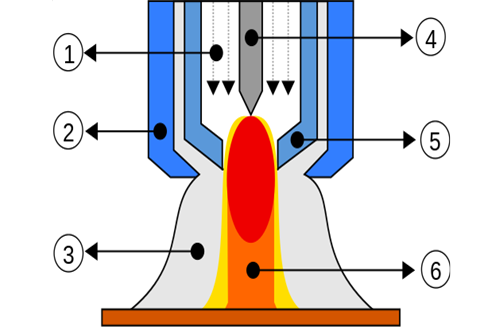
\includegraphics[width=\textwidth]{gorseller/ptaTorc}
\caption{PTA Torç}\label{fig:PtaTorc1}
\end{figure}
\lipsum[1-2]
\begin{table}
\centering
\caption{Deneme Tablosu.}\label{tab:den1}
\begin{tabular}{|l|l|l|}
\hline
sıra   & sayı   & toplam \\ \hline
1      & 2      & 3      \\ \hline
Kelime & deneme & son    \\ \hline
\end{tabular}
\end{table}


\section{Bulgular ve Tartışma Birinci Derece Başlık}
\lipsum[1-2]
\begin{figure}[h]
\centering
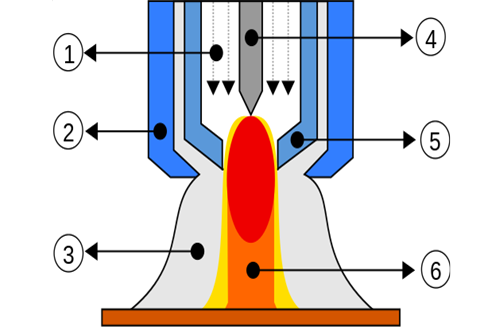
\includegraphics[width=\textwidth]{gorseller/ptaTorc}
\caption{PTA Torç}\label{fig:PtaTorc1}
\end{figure}
\lipsum[1-2]
\begin{table}
\centering
\caption{Deneme Tablosu.}\label{tab:den1}
\begin{tabular}{|l|l|l|}
\hline
sıra   & sayı   & toplam \\ \hline
1      & 2      & 3      \\ \hline
Kelime & deneme & son    \\ \hline
\end{tabular}
\end{table}
Teorem yazmak isterseniz:
\begin{theorem}[Öklid]
 İki noktadan bir ve yalnız bir doğru geçer.
\end{theorem}

İspat yazmak isterseniz:
\begin{ispat}[Tezin en önemli ispatı]
x=10
\end{ispat}

\subsection{Bulgular ve Tartışma ikinci derece başlık}
\lipsum[1-2]
\begin{figure}[h]
\centering
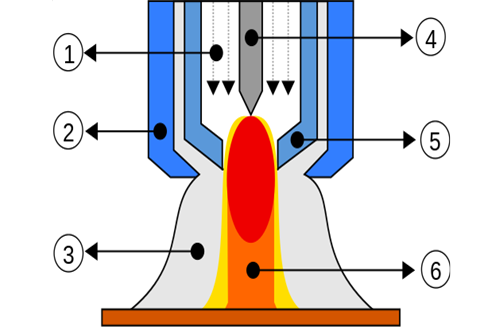
\includegraphics[width=\textwidth]{gorseller/ptaTorc}
\caption{PTA Torç}\label{fig:PtaTorc1}
\end{figure}
\lipsum[1-2]
\begin{table}
\centering
\caption{Deneme Tablosu.}\label{tab:den1}
\begin{tabular}{|l|l|l|}
\hline
sıra   & sayı   & toplam \\ \hline
1      & 2      & 3      \\ \hline
Kelime & deneme & son    \\ \hline
\end{tabular}
\end{table}

Teorem yazmak isterseniz:
\begin{theorem}[Öklid]
 İki noktadan bir ve yalnız bir doğru geçer.
\end{theorem}

İspat yazmak isterseniz:
\begin{ispat}[Tezin en önemli ispatı]
x=10
\end{ispat}

\subsubsection{Bulgular ve tartışma dördüncü derece başlık}
\lipsum[1-2]
\begin{figure}[h]
\centering
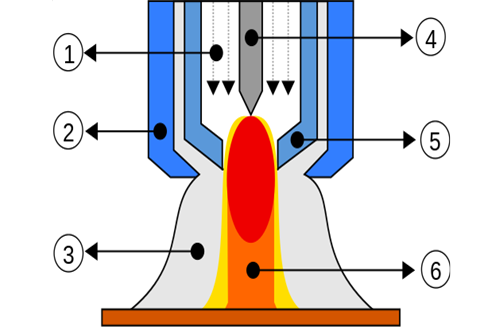
\includegraphics[width=\textwidth]{gorseller/ptaTorc}
\caption{PTA Torç}\label{fig:PtaTorc1}
\end{figure}
\lipsum[1-2]
\begin{table}
\centering
\caption{Deneme Tablosu.}\label{tab:den1}
\begin{tabular}{|l|l|l|}
\hline
sıra   & sayı   & toplam \\ \hline
1      & 2      & 3      \\ \hline
Kelime & deneme & son    \\ \hline
\end{tabular}
\end{table}

Teorem yazmak isterseniz:
\begin{theorem}[Öklid]
 İki noktadan bir ve yalnız bir doğru geçer.
\end{theorem}

İspat yazmak isterseniz:
\begin{ispat}[Tezin en önemli ispatı]
x=10
\end{ispat}
Eğer metin içinde \(\lim_{x \to \infty} \exp(-x) = 0\) ya da ortalayabilir
\begin{displaymath}
\cos (2\theta) = \cos^2 \theta - \sin^2 \theta
\end{displaymath}
isterseniz de numaralı denklem yazabilirsiniz.

\begin{equation}
\frac{\mathrm d}{\mathrm d x} \left( k g(x) \right)
\end{equation}
\subsubsection{Kimya}
\ce{B4C} yazabilirsiniz. Ya da

\ce{CO2 + C -> 2CO}

Daha fazlası için mhchem paketine bakınız.
 
\section{Analiz}
Eğer metin içinde şekile referans vermek isterseniz Şekil\ref{fig:PtaTorc} yazarsınız. 

Kaynakça böyle verilebilir \parencite{celik_microstructure_2013} ya da iki yazarlı ise böyle verilebilir \parencite{gatto_plasma_2004} veya ikiden fazla ise böyle verilebilir.
\parencite{celik_effects_2011}

Kaynakça listesi için daha çok referans verilmek istenirse \parencite{yazdi_microstructure_2015, keehan_influence_2006, guo_microstructure_2014}, \parencite{kim_variation_2013}, bir başkası \parencite{xibao_metallurgical_2005},  ya da başkası \parencite{jin_effect_1997} kullanılabilir.	
\chapter{Sonuçlar ve Öneriler}
\lipsum[1-3]

%\begin{figure}[h]
\caption{PTA Torç}\label{fig:PtaTorc}
\end{figure}
\begin{figure}[h]
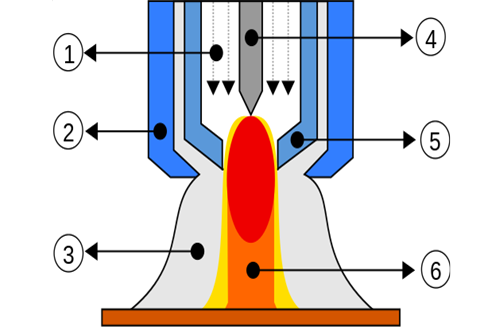
\includegraphics[width=\textwidth]{gorseller/ptaTorc}
\caption{PTA Torç}\label{fig:PtaTorc}
\end{figure}
\begin{figure}[h]
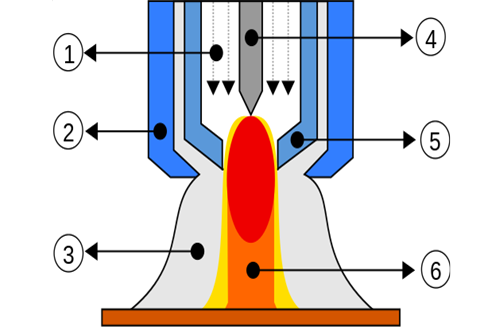
\includegraphics[width=\textwidth]{gorseller/ptaTorc}
\caption{PTA Torç}\label{fig:PtaTorc}
\end{figure}
\begin{figure}[h]
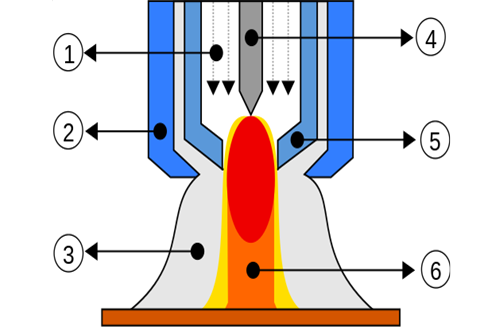
\includegraphics[width=\textwidth]{gorseller/ptaTorc}
\caption{PTA Torç}\label{fig:PtaTorc}
\end{figure}
\begin{figure}[h]
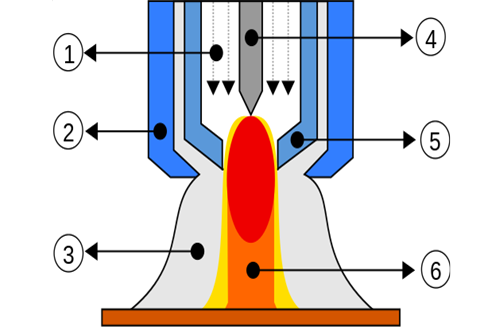
\includegraphics[width=\textwidth]{gorseller/ptaTorc}
\caption{PTA Torç}\label{fig:PtaTorc}
\end{figure}
\begin{figure}[h]
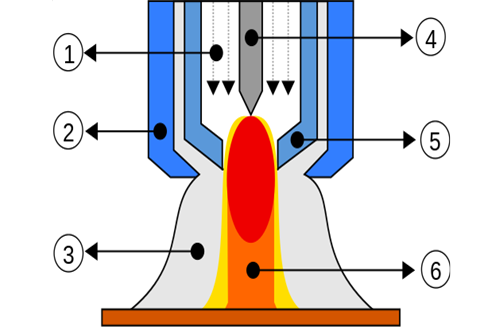
\includegraphics[width=\textwidth]{gorseller/ptaTorc}
\caption{PTA Torç}\label{fig:PtaTorc}
\end{figure}
\begin{figure}[h]
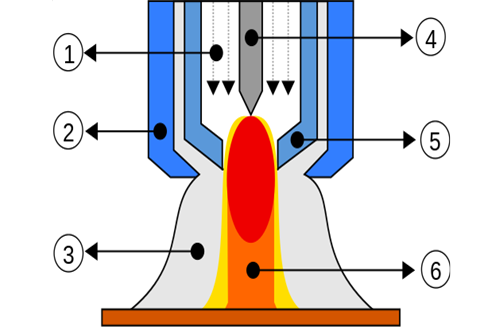
\includegraphics[width=\textwidth]{gorseller/ptaTorc}
\caption{PTA Torç}\label{fig:PtaTorc}
\end{figure}\begin{figure}[h]
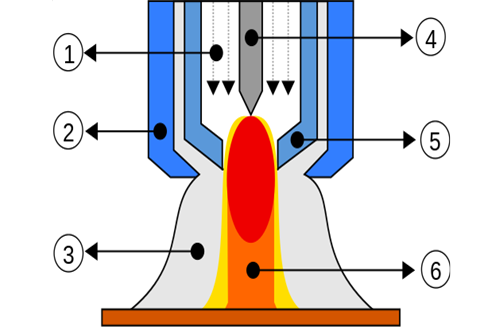
\includegraphics[width=\textwidth]{gorseller/ptaTorc}
\caption{PTA Torç}\label{fig:PtaTorc}
\end{figure}
\begin{figure}[h]
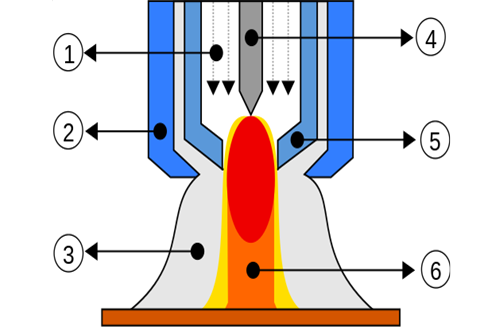
\includegraphics[width=\textwidth]{gorseller/ptaTorc}
\caption{PTA Torç}\label{fig:PtaTorc}
\end{figure}
\begin{figure}[h]
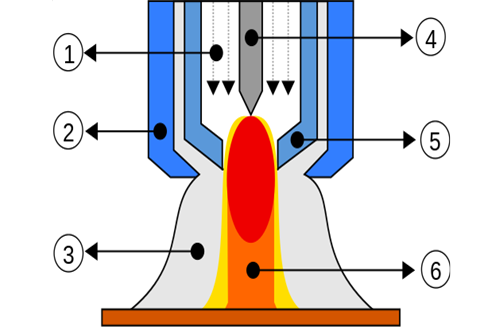
\includegraphics[width=\textwidth]{gorseller/ptaTorc}
\caption{PTA Torç}\label{fig:PtaTorc}
\end{figure}
\begin{figure}[h]
\caption{PTA Torç}\label{fig:PtaTorc}
\end{figure}


vfj ndsobvsfobşvjnsfbvs
 sjfdb s
\lipsum 

\begin{figure}[h]
\caption{PTA Torç}\label{fig:PtaTorc}
\end{figure}
\begin{figure}[h]
\caption{PTA Torç}\label{fig:PtaTorc}
\end{figure}
\begin{figure}[h]
\caption{PTA Torç}\label{fig:PtaTorc}
\end{figure}
\begin{figure}[h]
\caption{PTA Torç}\label{fig:PtaTorc}
\end{figure}
\begin{figure}[h]
\caption{PTA Torç}\label{fig:PtaTorc}
\end{figure}

\begin{figure}
\caption{PTA Torç}\label{fig:PtaTorc}
\end{figure}

\begin{figure}
\caption{PTA Torç}\label{fig:PtaTorc}
\end{figure}
vrebvsfdbsdbf

\begin{figure}
\caption{PTA Torç}\label{fig:PtaTorc}
\end{figure}

\begin{figure}
\caption{PTA Torç}\label{fig:PtaTorc}
\end{figure}
\cleardoublepage

\begin{figure}
\caption{PTA Torç}\label{fig:PtaTorc}
\end{figure}
\begin{figure}[h]
\caption{PTA Torç}\label{fig:PtaTorc}
\end{figure}
\begin{figure}[h]
\caption{PTA Torç}\label{fig:PtaTorc}
\end{figure}
\begin{figure}[h]
\caption{PTA Torç}\label{fig:PtaTorc}
\end{figure}
\section{d}

cdsvefvfdv
\begin{figure}[h]
\caption{PTA Torç}\label{fig:PtaTorc}
\end{figure}
\begin{figure}[h]
\caption{PTA Torç}\label{fig:PtaTorc}
\end{figure}
\begin{figure}[h]
\caption{PTA Torç}\label{fig:PtaTorc}
\end{figure}
\begin{figure}[h]
\caption{PTA Torç}\label{fig:PtaTorc}
\end{figure}
\begin{figure}[h]
\caption{PTA Torç}\label{fig:PtaTorc}
\end{figure}
\chapter{dsd}
\begin{figure}[h]
\caption{PTA Torç}\label{fig:PtaTorc}
\end{figure}
\section{fg}
\begin{figure}[h]
\caption{PTA Torç}\label{fig:PtaTorc}
\end{figure}
\begin{figure}[h]
\caption{PTA Torç}\label{fig:PtaTorc}
\end{figure}

\begin{figure}[h]
\caption{PTA Torç}\label{fig:PtaTorc}
\end{figure}
\newpage

\printbibliography[ title={KAYNAKLAR\space DİZİNİ}] %numaralı olsun istersen optionlarda heading=bibnumbered, yaz
\defbibheading{bibliography}[\refname]{%
  \section*{#1}%
  \markboth{\MakeUppercase{#1}}{\MakeUppercase{#1}}}
  
\noindent \addtocontents{toc}{\textbf{Özgeçmiş}}   % Sadece doktora tezleri için

\end{document}